\documentclass[11pt,letterpaper]{article}
\usepackage[T1]{fontenc}
\usepackage{lmodern}
\usepackage[margin=1in]{geometry}
\usepackage{amsmath,amssymb}
\usepackage{booktabs,tabularx,longtable,array,multirow}
\usepackage{graphicx}
\usepackage{xcolor}
\usepackage{tikz}
\usetikzlibrary{arrows.meta,positioning,fit,calc}
\usepackage{pgfplots}
\pgfplotsset{compat=1.18}
\usepackage{enumitem}
\usepackage{fancyhdr}
\usepackage{caption}
\usepackage{algorithm}
\usepackage{algpseudocode}
\usepackage{listings}
\usepackage{microtype}
\usepackage[section]{placeins}
\renewcommand{\topfraction}{0.9}
\renewcommand{\bottomfraction}{0.8}
\renewcommand{\textfraction}{0.07}
\renewcommand{\floatpagefraction}{0.75}
\setcounter{totalnumber}{5}
\setcounter{topnumber}{3}
\usepackage[hidelinks]{hyperref}

\captionsetup{font=small,labelfont=bf,labelsep=period}
\setlist{itemsep=2pt,topsep=3pt}
\renewcommand{\arraystretch}{1.15}
\newcolumntype{L}{>{\raggedright\arraybackslash}X}
\newcommand{\nd}{\textit{not documented}}
\newcommand{\pass}{pass}
\newcommand{\fail}{\textbf{fail}}
\newcommand{\ind}{\mathbb{1}}

\pagestyle{fancy}
\fancyhf{}
\fancyhead[L]{\small Evidence-Weighted Confidence}
\fancyhead[R]{\small Zeinoun $\cdot$ Preprint, October 2026}
\fancyfoot[C]{\small\thepage}
\renewcommand{\headrulewidth}{0.4pt}

\lstset{basicstyle=\ttfamily\footnotesize,columns=fullflexible,frame=none,breaklines=true,
  backgroundcolor=\color{black!4},xleftmargin=4pt,xrightmargin=4pt}

\begin{document}

\thispagestyle{empty}
\begin{center}
{\small Preprint $\cdot$ Method, analysis and experiments}\\[14pt]
{\LARGE\bfseries Evidence-Weighted Confidence}\\[4pt]
{\large Auditable, Calibrated Scoring of LLM Outputs}\\[14pt]
{\large Issam Zeinoun}\\
{Independent Researcher}\\
{October 2026}
\end{center}
\vspace{6pt}

\begin{abstract}
\noindent A confidence number reported by a large language model (LLM) has no defined meaning: nothing ties ``0.9'' to how often the model is right. We propose evidence-weighted confidence (EWC), a design pattern that replaces self-reported confidence with a score computed from verifiable evidence. A domain rubric, derived from the rules that govern the decision, breaks each output into evidence questions; for medical coding, those rules are the ICD-10-CM Official Guidelines for Coding and Reporting and the code's own instructional notes. The LLM answers each question and quotes the supporting source text; code verifies the quote, and a logistic regression fitted on labeled data turns the answers into a probability. Because the weights are log likelihood ratios, the score is a Bayesian posterior log-odds, and every score can be traced to the quotes behind it.

We test the pattern on ICD-10-CM E11.22 (type 2 diabetes with diabetic chronic kidney disease) in three pre-registered studies on synthetic outpatient charts, ending with a 350-chart study (150 development, 200 held-out test charts) on five models: GPT-5.4, Claude Sonnet 5.5, Claude Haiku 5.5, Gemini 3.8 Flash and Gemini 3.5 Flash-Lite. On the held-out test, EWC ranked charts better than the model's own stated confidence on every model (AUROC 0.897--1.000 against 0.593--0.772 after recalibration; every paired difference significant) and was the best-calibrated method on every model (expected calibration error 0.002--0.050). When EWC gave 90\% or more, the chart was supported 93--100\% of the time on all five models; when the models themselves said 93--99\%, they were right 54--72\% of the time. Giving the model the same questions and asking it to base its confidence on them closed the gap only for the two strongest models, and left GPT-5.4 confident at 97\% while it was right 60\% of the time. With EWC the two inexpensive models matched or approached the frontier models: Claude Haiku 5.5 reached AUROC 0.994 and ECE 0.014 at about one fifteenth of the cost of Claude Sonnet 5.5. The data are synthetic and their labels follow largely from the facts the rubric asks about, which favors the method; the results show that the pattern works as designed, not yet that it works on real charts.

\medskip\noindent\textbf{Keywords:} LLM evaluation; calibration; uncertainty; auditability; weight of evidence; logistic regression; medical coding; risk adjustment.
\end{abstract}

% ---------------------------------------------------------------------------
\section{Introduction}

A confidence score is a claim about frequency: of all outputs scored 0.9, about 90\% should be correct. A number the model writes in its answer makes no such claim, because nothing in its production was checked against outcomes. Empirical work confirms this. Xiong et al.~\cite{xiong} found that verbalized confidence clusters in the 80--100\% range in multiples of 5 and is poorly calibrated. Later work reports that RLHF-tuned models are more overconfident than their pre-RLHF versions~\cite{leng}. Leng et al.\ correct this during training. The method proposed here works at inference with any model and keeps the model's self-assessment out of the score, although bias can still reach the extraction step, which Section~\ref{sec:experiments} measures.

Asking the model to explain its reasoning does not fix this. A written rationale is more text, not a measurement, and two rationales cannot be compared on a numeric scale. In regulated domains the problem is practical as well as statistical. A payer that auto-accepts a diagnosis code at ``95\% confidence'' must be able to show an auditor why, and must know that the 95\% means something.

Medical coding makes the stakes concrete. Soroush et al.~\cite{soroush} found that GPT-4, the best model tested, reproduced the exact ICD-10-CM code less than half the time. Accuracy will improve, but no accuracy level removes the need to know which individual outputs to trust. Their study generated codes from code descriptions; this paper addresses a different task, scoring a candidate code against the full chart, and does not aim to improve coding accuracy itself.

\paragraph{Contributions.} The main contribution is a design pattern: an LLM reads the source and answers rule-derived questions with verified quotes, and a small statistical model on top turns the answers into a calibrated probability. The paper makes four specific contributions:
\begin{enumerate}
  \item \textbf{The method} (Sections~\ref{sec:method}--\ref{sec:example}): a decomposition of an LLM decision into evidence questions with cited, machine-verified answers, scored by deterministic code, with a Bayesian interpretation in which rubric weights are log likelihood ratios.
  \item \textbf{Evidence that the confidence it gives means what it says} (Section~\ref{sec:results-calib}): on held-out charts and five models, the score's stated probability matched the observed rate of supported charts, while the models' own confidence did not.
  \item \textbf{Evidence that tuning the questions, not the model, fixes errors} (Section~\ref{sec:results-tuning}): a failure found on charts outside the original rubric was fixed by adding two rule-derived questions, with no change to any model.
  \item \textbf{Evidence that the pattern lets inexpensive models do the job} (Section~\ref{sec:results-cost}): with EWC, Claude Haiku 5.5 and Gemini 3.5 Flash-Lite outperformed the stated confidence of every frontier model tested, and Haiku matched the best of them.
\end{enumerate}
A calibration and evaluation protocol (Section~\ref{sec:protocol}) and a full algorithm specification (Appendix~\ref{app:algo}) make the method reproducible.

\FloatBarrier
\subsection{What the method adds to LLM validation}\label{sec:adds}

The method targets the two main failures of current LLM validation: opacity, meaning no account of why an output was produced, and miscalibration, meaning no defined meaning behind the confidence number. It is designed to add four things; Section~\ref{sec:experiments} reports how each fared.
\begin{enumerate}
  \item \textbf{Calibrated confidence instead of a verbalized guess.} Verbalized confidence clusters between 80\% and 100\% and is poorly calibrated against observed accuracy~\cite{xiong}. Here the score is a sum of log likelihood ratios with weights fitted by logistic regression, so it is a probability that can be tested against outcomes (Sections~\ref{sec:bayes} and~\ref{sec:protocol}).
  \item \textbf{An auditable trail instead of a black box.} Every score comes with the structured rubric answers and the source quotes behind them, and code checks each quote against the document. A reviewer can see exactly which evidence raised or lowered the score (Section~\ref{sec:method}).
  \item \textbf{Silence and contradiction kept apart.} Binary checklist judges and yes/no checks merge ``the source does not say'' with ``the source says the opposite.'' The three-way answer (yes, no, \nd) gives each its own weight. The distinction matters in clinical, legal and financial review, where a missing statement and a contrary statement lead to different decisions (Section~\ref{sec:example}, question Q3).
  \item \textbf{Threshold routing on a real probability.} Because the score is calibrated, an organization can route on it, accepting high-scoring outputs automatically and sending the rest to human review. Where to set the thresholds is an operational choice made from calibration data, which balances throughput against compliance risk.
\end{enumerate}

% ---------------------------------------------------------------------------
\section{Related work}

Evidence-weighted confidence builds on the work summarized in Table~\ref{tab:related}; none of it alone yields an auditable, calibrated score for each LLM output. The last column states what this paper adds; Section~\ref{sec:experiments} tests these additions on synthetic data.

The contribution is the combination: an LLM as the concept extractor, a verified citation for every concept, and a classical scorecard on top. The closest analogue is the concept bottleneck model, with the bottleneck made explicit, human-authored, and checked against the source document.

\begin{table}[!htbp]
\centering\small
\caption{Related work, its limits for this problem, and what this paper adds.}\label{tab:related}
\begin{tabularx}{\textwidth}{@{}p{2.3cm}LLL@{}}
\toprule
Line of work & What it does & What it lacks for this problem & What this paper adds \\
\midrule
Verbalized and logit confidence~\cite{xiong,leng}; post-hoc recalibration~\cite{platt} & Asks the model for a number, or reads token probabilities; Platt or isotonic mapping can recalibrate it & Overconfident, more so after RLHF; no evidence trail; cannot be decomposed or audited & A score computed from verified evidence instead of self-assessment; recalibrated verbalized confidence serves as a baseline \\
Checklist LLM judges, e.g.\ CheckEval~\cite{checkeval} & Breaks evaluation into yes/no questions; improves agreement across judge models & Built for grading text quality; aggregation is a plain count, not a probability & Weights fitted to outcomes as log likelihood ratios; a third answer for \nd; quote verification \\
Concept bottleneck models~\cite{cbm} & Predicts human-readable concepts first, then the label from the concepts & Needs concept labels to train the concept predictor & A pre-trained LLM extracts concepts with cited quotes, so only outcome labels are needed (shown here with about 100 labeled charts) \\
Weight-of-evidence scorecards and clinical scores~\cite{good} & Adds points per finding as log-odds; fitted by logistic regression & Assume structured inputs; no method for unstructured text & The same scoring theory applied to evidence an LLM extracts from text and code verifies \\
LLM medical coding benchmarks~\cite{soroush} & Measure how often a model produces the correct code & Overall accuracy does not say which individual outputs to trust & A per-output probability for a candidate code; no claim to improve coding accuracy \\
AI monitoring in prior authorization~\cite{zeinoun} (same author) & Label-based and label-free monitoring, a batch AI critic, a risk model for human scrutiny & Monitors the workflow over time; no calibrated probability per output & A per-output probability from criterion-level evidence, usable as an input to that monitoring \\
\bottomrule
\end{tabularx}
\end{table}

% ---------------------------------------------------------------------------
\section{Method}\label{sec:method}

The method separates reading from judging: the LLM reads the source and answers questions, and deterministic code turns the answers into a score (Figure~\ref{fig:pipeline}).

\paragraph{Rubric.} For each candidate output (here, a diagnosis code), a rubric defines a set of evidence questions. Each question has one of two roles:
\begin{itemize}
  \item \textbf{Gate questions} must be answered yes for the output to be valid at all, like a prior-authorization criterion. A failed gate sets the score to zero.
  \item \textbf{Weighted questions} shift confidence up or down once the gates pass.
\end{itemize}
Each question has three possible answers: yes, no (the source contradicts it), and \nd{} (the source is silent). The three carry separate weights, because contradiction and silence are different evidence. Breaking a judgment into yes/no questions follows checklist evaluators such as CheckEval~\cite{checkeval}, which showed that it makes LLM judges agree more and their scores easier to interpret. CheckEval grades text quality and counts its answers; this method scores factual support against a source document, adds the third answer, and fits a weight to each answer.

\begin{figure}[!htbp]
\centering
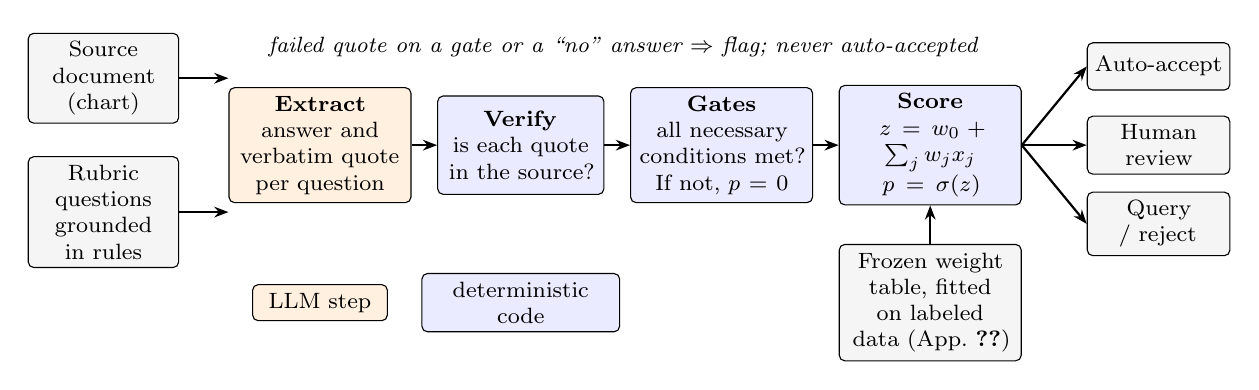
\begin{tikzpicture}[font=\footnotesize,
  box/.style={draw,rounded corners=2pt,align=center,inner sep=3pt,minimum height=1.25cm},
  llm/.style={box,fill=orange!12},
  det/.style={box,fill=blue!8},
  plain/.style={box,fill=black!4},
  arr/.style={-{Stealth[length=1.8mm]},thick}]
\node[plain,text width=1.7cm,minimum height=0.9cm] (src) at (0,0.85) {Source document (chart)};
\node[plain,text width=1.7cm,minimum height=0.9cm] (rub) at (0,-0.85) {Rubric questions grounded in rules};
\node[llm,text width=2.1cm] (ext) at (2.75,0) {\textbf{Extract}\\answer and verbatim quote per question};
\node[det,text width=1.9cm] (ver) at (5.3,0) {\textbf{Verify}\\is each quote in the source?};
\node[det,text width=2.1cm] (gate) at (7.85,0) {\textbf{Gates}\\all necessary conditions met? If not, $p=0$};
\node[det,text width=2.1cm] (score) at (10.5,0) {\textbf{Score}\\$z=w_0+\sum_j w_j x_j$\\$p=\sigma(z)$};
\node[plain,text width=2.1cm,minimum height=0.9cm] (wt) at (10.5,-2.0) {Frozen weight table, fitted on labeled data (App.~\ref{app:algo})};
\node[plain,text width=1.6cm,minimum height=0.6cm] (acc) at (13.4,1.0) {Auto-accept};
\node[plain,text width=1.6cm,minimum height=0.6cm] (rev) at (13.4,0) {Human review};
\node[plain,text width=1.6cm,minimum height=0.6cm] (rej) at (13.4,-1.0) {Query / reject};
\draw[arr] (src.east) -- (ext.west|-src.east); \draw[arr] (rub.east) -- (ext.west|-rub.east);
\draw[arr] (ext) -- (ver); \draw[arr] (ver) -- (gate); \draw[arr] (gate) -- (score);
\draw[arr] (wt) -- (score);
\draw[arr] (score.east) -- (acc.west); \draw[arr] (score.east) -- (rev.west); \draw[arr] (score.east) -- (rej.west);
\node[font=\footnotesize\itshape,align=center] at (6.6,1.25) {failed quote on a gate or a ``no'' answer $\Rightarrow$ flag; never auto-accepted};
\node[llm,minimum height=0.45cm,text width=1.5cm] at (2.75,-2.0) {LLM step};
\node[det,minimum height=0.45cm,text width=2.3cm] at (5.3,-2.0) {deterministic code};
\end{tikzpicture}
\caption{The evidence-weighted confidence pipeline. Only extraction uses an LLM; verification, gates, scoring and routing are deterministic and logged, so every score can be reproduced from its evidence.}\label{fig:pipeline}
\end{figure}

\paragraph{Grounding.} Questions are derived from the authoritative rules that govern the decision rather than written freely: the official coding guidelines for medical coding, the payer's medical policy for prior authorization, and payment policy for overpayment review. Each question records the rule it implements and that rule's version. The score then measures whether the documentation meets the rules the decision is held to, and a rubric change can be traced to a rule change. Section~\ref{sec:grounding} shows the mapping for E11.22.

\paragraph{Pipeline.}
\begin{enumerate}
  \item \textbf{Extract.} The LLM receives the source document and the rubric questions, without the weights. For each question it returns an answer and, for yes or no, the exact quote that supports it.
  \item \textbf{Verify.} Code checks every quote against the source with a plain string match: after case and spacing are normalized, the quote must appear word for word in the document. It is a string search, not a regular expression, because clinical text is full of characters (parentheses, periods, slashes, plus signs) that a regular expression would treat as commands. An answer whose quote is not found is downgraded to \nd. Downgrading is conservative only for evidence that would raise the score; for a contradiction it would remove a penalty. So when a gate answer or a no answer fails verification, the chart is also flagged for human review and cannot be auto-accepted, whatever its score.
  \item \textbf{Score.} Code looks up the weight for each verified answer, adds the intercept, and converts the total from log-odds to a probability.
  \item \textbf{Log.} The record stores answers, quotes, rubric version, weight-table version and score, so any score can be reproduced later.
\end{enumerate}
An extraction record looks like this:
\begin{lstlisting}
{"question": "ckd_stage_documented", "answer": "yes",
 "quote": "CKD stage 3a, stable", "verified": true}
\end{lstlisting}

The separation has three practical consequences. First, score variance across repeated runs comes only from extraction, which can be measured question by question. Second, a hallucinated piece of evidence fails verification instead of raising the score. Third, a new weight table can be applied to every historical record without new LLM calls, which makes calibration cheap. The structure resembles a concept bottleneck model~\cite{cbm}, which predicts human-readable concepts and then the label from them. The difference is the extractor: concept bottleneck models train a concept predictor on concept labels, while here a pre-trained LLM extracts the concepts with cited quotes. Only outcome labels are then needed to fit the weights; in the experiments, about 100 labeled development charts per model were enough.

% ---------------------------------------------------------------------------
\section{Bayesian foundation}\label{sec:bayes}

Adding points per finding is exact Bayesian updating when the points are log likelihood ratios. Let $C$ be the event that the output is correct and $e_1,\dots,e_n$ the verified answers. Bayes' rule in odds form is
\begin{equation}
\frac{P(C\mid e_1,\dots,e_n)}{P(\neg C\mid e_1,\dots,e_n)} = \frac{P(C)}{P(\neg C)}\prod_{i=1}^{n}\frac{P(e_i\mid C)}{P(e_i\mid \neg C)}.
\end{equation}
The product holds when the answers are conditionally independent given $C$. Taking logs turns it into a sum:
\begin{equation}
\operatorname{logit} P(C\mid e) = w_0 + \sum_{i=1}^{n} w_i(e_i),\qquad w_0=\log\frac{P(C)}{P(\neg C)},\qquad w_i(e_i)=\log\frac{P(e_i\mid C)}{P(e_i\mid\neg C)}.
\end{equation}
The intercept $w_0$ is the prior: how often the output is correct before reading the evidence. Each weight $w_i$ is the weight of evidence of one answer~\cite{good}. This is the theory behind weight-of-evidence scorecards and clinical point scores, which fit their points by logistic regression and commonly give missing values their own bin. Those tools assume structured inputs; the contribution here is applying them to evidence an LLM extracts from unstructured text and code verifies. The three-way answer adapts the missing-value bin rather than introducing a new idea. Four consequences follow.
\begin{enumerate}
  \item \textbf{Scores compose without overflow.} Adding ``+30\%'' per finding can exceed 100\%. Log-odds are unbounded and map back to a probability between 0 and 1.
  \item \textbf{Absence of evidence counts.} If a finding is common among correct outputs, its absence has a likelihood ratio below 1 and a negative weight. A rubric that only adds points for findings ignores this. With silence as the zero point (below), the same fact shows up as a larger weight for yes.
  \item \textbf{Correlated evidence is double-counted.} Two answers that restate one fact (a CKD diagnosis in the problem list and in the assessment) violate independence and inflate the score. This is the known weakness of naive Bayes.
  \item \textbf{Logistic regression fixes point 3.} Logistic regression has the same additive log-odds form but fits all weights jointly, so correlated answers share credit. Its coefficients are the calibrated weights. The price is that a single fitted weight no longer reads as the strength of one piece of evidence on its own; Section~\ref{sec:results-weights} shows an example.
\end{enumerate}
The method therefore has two stages. Expert-assigned weights give a usable, auditable score on day one. Fitted weights turn that score into a probability that can be tested.

In practice the weights are written with silence as the zero point: every \nd{} answer counts 0, and its effect is absorbed into the starting score $w_0$. Predictions are unchanged, but $w_0$ then means the log-odds for a chart that passes the gates and documents nothing further, rather than the population base rate. This is the only form used in the rest of the paper, because it is the form logistic regression can fit uniquely (Appendix~\ref{app:algo}).

% ---------------------------------------------------------------------------
\section{Worked example: E11.22}\label{sec:example}

E11.22 (type 2 diabetes mellitus with diabetic chronic kidney disease) shows gates, three-way answers and a contradiction in one rubric (Table~\ref{tab:rubric}). The weights are illustrative, not fitted. Silence (\nd) counts 0 on every question. The starting score is $w_0=-4.30$: the log-odds for a chart that passes the gates but documents nothing beyond them. Each answer then adds to or subtracts from that starting score. The rubric used in the final experiment (version 3) adds two gates for the encounter and the signature; Appendix~\ref{app:rubric} lists it in full.

\begin{table}[!htbp]
\centering\small
\caption{Illustrative E11.22 rubric. Weights are added to the starting score $w_0=-4.30$; silence is the zero point.}\label{tab:rubric}
\begin{tabularx}{\textwidth}{@{}Llccc@{}}
\toprule
Question & Role & Yes & No (contradicted) & Not documented \\
\midrule
G1. Type 2 diabetes documented in the encounter note & Gate & pass & fail & fail \\
G2. Chronic kidney disease documented & Gate & pass & fail & fail \\
Q1. CKD stage documented & Weighted & $+2.19$ & n/a & 0 \\
Q2. eGFR below 60 on two results 90+ days apart & Weighted & $+1.40$ & $-1.20$ & 0 \\
Q3. Provider attributes CKD to diabetes & Weighted & $+0.90$ & $-2.00$ & 0 \\
Q4. Kidney disease monitored, evaluated, assessed or treated this encounter (MEAT) & Weighted & $+2.20$ & n/a & 0 \\
\bottomrule
\end{tabularx}
\end{table}

Q3 shows why three answers matter. ICD-10-CM's ``with'' convention presumes a link between diabetes and CKD unless the provider documents another cause, so silence costs nothing (0). An explicit statement adds evidence ($+0.90$). A documented other cause, such as hypertensive kidney disease, is strong evidence against the code ($-2.00$).

\FloatBarrier
\subsection{Grounding the rubric in the coding guidelines}\label{sec:grounding}

Every E11.22 question implements a specific rule from the ICD-10-CM Official Guidelines for Coding and Reporting (FY 2027, effective October 1, 2026)~\cite{guidelines} or from the code's instructional note in the Tabular List~\cite{tabular}. Under HIPAA, adherence to these guidelines is required when assigning diagnosis codes~\cite{guidelines}. A threshold on the score therefore measures how well the documentation meets rules coders are already held to, rather than how closely the note's wording resembles a code description (Table~\ref{tab:sources}).

\begin{table}[!htbp]
\centering\small
\caption{Source of each E11.22 rubric question.}\label{tab:sources}
\begin{tabularx}{\textwidth}{@{}p{2.2cm}p{2.1cm}LL@{}}
\toprule
Question & Source & What the source says & How the question applies it \\
\midrule
G1. Type 2 diabetes documented & Categories E10 and E11; Section I.C.4.a~\cite{guidelines} & Diabetes codes are combination codes classified by type: E11 is type 2, E10 is type 1. When the type is not documented, the default is E11 & A type 1 chart belongs under E10.22, so the gate fails. Diabetes documented without a type counts as yes \\
G2. CKD documented as an established diagnosis & Sections IV.H, IV.J and I.B.14~\cite{guidelines} & Outpatient: ``Do not code diagnoses documented as `probable', `suspected,' `questionable,' `rule out' '' or similar terms. Code coexisting conditions that affect care, but not ``conditions that were previously treated and no longer exist.'' Code assignment is based on the provider's documentation & Possible or rule-out CKD fails. Resolved acute kidney injury fails. Low eGFR values without a provider's CKD diagnosis fail \\
Q1. CKD stage documented & E11.22 instructional note~\cite{tabular} & ``Use additional code to identify stage of chronic kidney disease (N18.1--N18.6)'' & Rewards a documented stage. E11.22 remains assignable without one, so Q1 is weighted rather than a gate \\
Q2. eGFR below 60 on two results 90+ days apart & Section I.A.19~\cite{guidelines} & ``Code assignment is not based on clinical criteria used by the provider to establish the diagnosis'' & Lab support is not a coding requirement, so Q2 is weighted rather than a gate. It reflects clinical validation, a separate review that payers and auditors apply \\
Q3. Provider attributes CKD to diabetes & Section I.A.15, ``With''~\cite{guidelines} & The classification ``presumes a causal relationship'' between conditions linked by ``with'', even without explicit provider linkage, ``unless the documentation clearly states the conditions are unrelated'' & Silence costs nothing (weight 0). An explicit link adds evidence. A documented other cause rebuts the presumption and carries a strong negative weight \\
Q4. CKD addressed this encounter & Sections IV.I and IV.J~\cite{guidelines}; MEAT audit convention & Chronic diseases ``treated on an ongoing basis may be coded and reported as many times as the patient receives treatment and care''; code conditions ``that require or affect patient care, treatment or management'' & Requires evidence that CKD was monitored, evaluated, assessed or treated at this visit. MEAT is an industry risk-adjustment audit convention, not text from the Official Guidelines \\
\bottomrule
\end{tabularx}
\end{table}

Three rules shape the E11.22 rubric most:
\begin{enumerate}
  \item \textbf{Linkage is presumed unless contradicted.} Section I.A.15 presumes a causal relationship between diabetes and chronic kidney disease when they occur ``with'' each other. The presumption holds unless the documentation clearly states the conditions are unrelated. Q3 tests whether the link is present, absent or contradicted, and only a contradiction counts against the code.
  \item \textbf{The code calls for a stage.} The instructional note for E11.22 requires an additional code for the CKD stage from N18.1--N18.6. Q1 checks whether the note documents the stage needed for that companion code.
  \item \textbf{The diagnosis must be certain and current.} Outpatient guidelines exclude uncertain diagnoses and conditions that no longer exist, and code assignment rests on the provider's documentation. G2 therefore rejects rule-out impressions, resolved conditions and diagnoses inferred from labs alone.
\end{enumerate}
The mapping is the author's reading of the guidelines. It has not yet been reviewed by a certified coder, and payer policy or official coding advice may add requirements.

\FloatBarrier
\subsection{Three charts}

Table~\ref{tab:three} scores three charts that all pass the gates, and Figure~\ref{fig:logistic} places them on the logistic curve.

\begin{table}[!htbp]
\centering\small
\caption{Three charts scored with the illustrative weights of Table~\ref{tab:rubric}. n.d.\ = not documented.}\label{tab:three}
\begin{tabularx}{\textwidth}{@{}p{3.2cm}p{3.2cm}Lc@{}}
\toprule
Chart & Verified answers & Log-odds & Probability \\
\midrule
A. Complete documentation & Q1 yes, Q2 yes, Q3 yes, Q4 yes & $-4.30+2.19+1.40+0.90+2.20=2.39$ & 0.92 \\
B. Problem-list mention only & Q1 yes, Q2 n.d., Q3 n.d., Q4 n.d. & $-4.30+2.19+0+0+0=-2.11$ & 0.11 \\
C. CKD attributed to hypertension & Q1 yes, Q2 yes, Q3 no, Q4 yes & $-4.30+2.19+1.40-2.00+2.20=-0.51$ & 0.38 \\
\bottomrule
\end{tabularx}
\end{table}

\begin{figure}[!htbp]
\centering
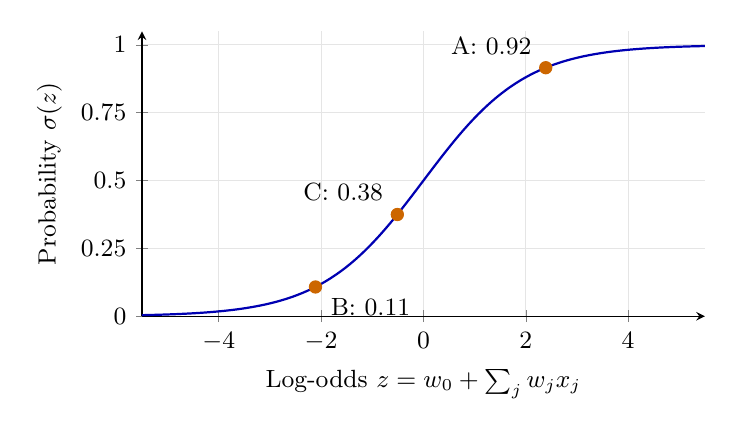
\begin{tikzpicture}
\begin{axis}[width=0.72\textwidth,height=5.2cm,xmin=-5.5,xmax=5.5,ymin=0,ymax=1.05,
  xlabel={Log-odds $z=w_0+\sum_j w_j x_j$},ylabel={Probability $\sigma(z)$},
  ytick={0,0.25,0.5,0.75,1},axis lines=left,grid=major,grid style={black!10},font=\small]
\addplot[domain=-5.5:5.5,samples=120,thick,blue!70!black]{1/(1+exp(-x))};
\addplot[only marks,mark=*,mark size=2.2pt,orange!80!black] coordinates {(2.39,0.916) (-2.11,0.108) (-0.51,0.375)};
\node[anchor=south east,font=\small] at (axis cs:2.3,0.93) {A: 0.92};
\node[anchor=north west,font=\small] at (axis cs:-2.0,0.10) {B: 0.11};
\node[anchor=south east,font=\small] at (axis cs:-0.6,0.39) {C: 0.38};
\end{axis}
\end{tikzpicture}
\caption{The three charts of Table~\ref{tab:three} on the logistic curve. Each chart's evidence adds up to a log-odds score $z$, and the sigmoid turns it into a probability. The same change in evidence moves the probability most in the middle of the curve and least at the extremes.}\label{fig:logistic}
\end{figure}

An LLM asked for a confidence number might rate all three charts 85--95\%, because each mentions both diabetes and CKD; the experiments below show that this is what happens (Section~\ref{sec:results-calib}). The rubric separates them, and each score comes with the quotes that produced it. Chart B is the typical unsupported diagnosis in a risk-adjustment audit: carried in the problem list but not addressed in the visit. Chart C would likely be coded differently by a human coder.

With calibrated weights, the score supports threshold routing (Section~\ref{sec:adds}). Thresholds are an operational choice made from calibration data to meet a target precision and reviewer workload; the experiments use a target of 95\% precision chosen on development data.

% ---------------------------------------------------------------------------
\section{Calibration and evaluation protocol}\label{sec:protocol}

The claim that a score is a probability is falsifiable, and this protocol tests it.

\paragraph{Data.} A labeled set of (document, candidate code, correct or not) triples, ideally labeled by certified coders, with inter-rater agreement reported. Public options include synthetic notes or de-identified notes such as MIMIC; a rough sample-size rule is 10--20 positive cases per fitted weight.

\paragraph{Fitting.}
\begin{enumerate}
  \item Run extraction once on all documents and store the verified answers.
  \item Encode each answer as indicator features: yes and no per question, with \nd{} as the zero point.
  \item Fit L2-regularized logistic regression on a training split. For rare codes, fit at the family level and let each code deviate slightly (partial pooling; see Section~\ref{sec:general}).
  \item Score the held-out split with the fitted weight table.
\end{enumerate}
Appendix~\ref{app:algo} specifies the encoding, objective, regularization search and prior adjustment precisely enough to reimplement.

\paragraph{Metrics.} Table~\ref{tab:metrics} lists what is measured.

\begin{table}[!htbp]
\centering\small
\caption{Evaluation metrics.}\label{tab:metrics}
\begin{tabularx}{\textwidth}{@{}p{3cm}L@{}}
\toprule
Property & Metric \\
\midrule
Calibration & Expected calibration error (ECE), Brier score, reliability diagram \\
Discrimination & AUROC \\
Operational value & Share of outputs auto-accepted at a target precision (coverage at precision) \\
Decision quality & Precision (headline), recall and $F_{0.5}$ at the auto-accept threshold chosen on the development split and applied unchanged to the test split, and at a fixed 0.5 threshold \\
Extraction quality & Criterion level, per question: precision and recall for each answer type, macro-$F_1$, and a confusion matrix against reference answers \\
Reproducibility & Score standard deviation over repeated extraction runs of the same document \\
Faithfulness & Share of quotes that fail verification, overall and per question; share of yes answers a coder rejects \\
\bottomrule
\end{tabularx}
\end{table}

Plain accuracy is not used as a headline metric. For the final decision, calibration and AUROC evaluate the probability itself, and threshold metrics are reported only at fixed operating points. $F_{0.5}$ is chosen because it weights precision over recall: for a payer, accepting an unsupported code risks recovery in an audit, while missing a supported one costs less. A use case with the opposite priority would report $F_2$. For extraction, answer types are imbalanced (a documented contradiction is far rarer than silence), so a model that always answered \nd{} could score well on agreement while missing every contradiction. Per-class recall and macro-$F_1$ expose that failure.

\paragraph{Baselines.}
\begin{enumerate}
  \item Verbalized confidence: the model reports a number directly.
  \item Verbalized confidence after post-hoc Platt~\cite{platt} or isotonic recalibration, the strongest existing comparison. Platt scaling maps one score to a probability after the fact; the method instead fits a weight to each piece of evidence, which keeps the score decomposable.
  \item Criteria-guided confidence: the model receives the same rubric questions and guidance and is told to base its confidence on them, but reports a single number. This isolates what the deterministic scoring adds beyond the questions themselves.
  \item Self-consistency: agreement rate across several sampled answers.
  \item The rubric with expert weights, unfitted.
  \item The rubric with the LLM computing the score itself.
\end{enumerate}

\paragraph{Ablations.} Remove span verification; collapse three-way answers to two; drop gates; fit naive Bayes instead of logistic regression to measure the cost of the independence assumption.

The central hypothesis is that the fitted rubric matches or beats recalibrated verbalized confidence on ECE and AUROC while adding a verified evidence trail. If it matches without beating, the evidence trail alone justifies it in audited settings.

% ---------------------------------------------------------------------------
\section{Experiments}\label{sec:experiments}

\FloatBarrier
\subsection{Overview}

The method was tested in three studies on synthetic outpatient charts, each pre-registered before its test data were run, with hypotheses, pass marks and analysis rules fixed in advance and every change logged with its date and reason. In each study the prompts, the rubric, the fitted weights, the recalibration maps and the auto-accept thresholds were frozen with cryptographic hashes before any test call, and the code refused to evaluate a model's test split more than once.

\begin{enumerate}
  \item \textbf{Study 1, pilot} (200 charts; 140 development, 60 test; GPT-5.4 and Gemini 3.8 Flash). The six-question rubric of Section~\ref{sec:example} on 13 scenarios.
  \item \textbf{Study 2, transfer test} (300 harder charts, frozen study-1 pipeline, no refitting; same two models). Stopped after its first stage of 100 charts, as its pre-registration allowed, once that stage had shown what the rubric missed.
  \item \textbf{Study 3, main study} (350 charts; 150 development, 200 test; five models). Rubric version 3, which adds two gates the study-2 failures called for. All headline results in this section come from study 3.
\end{enumerate}

\FloatBarrier
\subsection{Study 3 design}

\paragraph{Data.} 350 synthetic outpatient notes, each scored against the candidate code E11.22. Three hundred come from study 2's generator (median length about 3,400 characters, with format noise such as line breaks inside sentences, OCR-style character swaps and copied-forward sections), in seven scenario families:
A, the pilot scenarios rewritten (complete documentation, problem-list-only CKD, other causes, uncertain CKD, acute kidney injury, labs only);
B, copied-forward plans;
C, harder gates (untyped diabetes, insulin-treated type 2, type 1 in the history only, secondary diabetes, a history of CKD that is managed today, CKD resolved after transplant);
D, lab and date edge cases for the eGFR question;
E, cause attribution (diabetes named with another cause, hedged attribution, attribution only in a prior visit);
F, failures the pilot rubric could not see (a visit with a nurse or dietitian only, an unsigned note or a signature without a credential, a chart-review e-consult with no patient seen); and
G, borderline wording for ``addressed'' (``renal function reviewed, stable'', ``see nephrology note'', a medication change for kidney function without the word CKD, CKD in a reviewed list of chronic conditions).
Fifty new hard cases form family H: conflicting statements within a note, a stated stage that the labs contradict, end-stage renal disease and dialysis, and unclear or partial statements. Three of them deliberately keep a doubled phrase (``not on dialysis not on dialysis'') to see whether it confuses the models.

\paragraph{Labels.} A chart is supported (label 1) only if type 2 diabetes is documented (untyped defaults to type 2; secondary diabetes is not type 2); CKD is an established diagnosis; CKD is addressed at this visit; CKD is not attributed to another cause \emph{instead of} diabetes; the patient was seen face to face by an MD, DO, NP or PA; and the note is signed with a credential. ``Addressed'' follows the MEAT reading set by the study lead: a copied plan line with a status (``stable'', ``continue regimen'') and CKD in a reviewed list of chronic conditions count; ``see nephrology note'' alone does not; a medication change because of kidney function does. A contradiction about whether CKD exists, or about the diabetes type, that the note does not resolve makes the chart unsupported, because it calls for a provider query; a contradiction only about the stage does not. The rules were set by the study lead with AI assistance. A built-in checker that reads only the note text found 0 of 350 charts with problems and caught 6 of 6 planted errors, and the study lead reviewed 74 charts in two rounds, using Gemini 3.1 Pro as a reading aid. The development split has 150 charts (81 supported) and the test split 200 (117 supported); the test split holds 175 charts no model had seen and 25 unseen hard cases.

\paragraph{Methods compared.}
\begin{itemize}
  \item \textbf{A, stated confidence.} The model reads the chart and gives a 0--100 confidence that it supports E11.22; reported raw and after Platt recalibration fitted on development data. Five runs per chart; the first is scored.
  \item \textbf{B, evidence-weighted confidence.} The model answers the eight rubric-v3 questions with quotes (Appendix~\ref{app:rubric}); code verifies the quotes, applies the four gates (G1, G2, R1, R2) and scores Q1--Q4 with weights fitted on development data (Appendix~\ref{app:algo}). Five extraction runs per chart; the first is scored.
  \item \textbf{C, criteria-guided confidence.} The model receives the same eight questions and their guidance, is told to answer each for itself and base its confidence on them, and returns a single 0--100 number. One run per chart; not recalibrated.
\end{itemize}
Method C is the fair comparison for B: both see exactly the same questions, so any difference comes from how the answers become a number (verified quotes and a fitted model, against the LLM's own judgment).

\paragraph{Models.} GPT-5.4 (\texttt{gpt-5.4-2026-03-05}) and Gemini 3.8 Flash were pre-registered. Claude Sonnet 5.5, Claude Haiku 5.5 and Gemini 3.5 Flash-Lite were added afterwards, each under a written addendum filed before its first call, with its own development fit, its own freeze and a single test evaluation. Haiku and Flash-Lite were added to test whether the pattern lets inexpensive models do the job. Each model made 11 calls per chart: 2,200 test calls per model, all completed without errors.

\paragraph{Hypotheses (per model, test split).} 95\% intervals from 2,000 paired bootstrap resamples.
H1: B ranks better than recalibrated A by at least 0.10 AUROC, with the paired interval above 0.
H2: B ranks better than C, with the paired interval above 0.
H3: B's ECE is no higher than recalibrated A's and C's.
H4: B's auto-accept threshold, chosen on development data for 95\% precision, gives at least 95\% precision on test.
The pre-registration predicted in advance that H2 would likely fail for Gemini 3.8 Flash, where C had tied B on development data.

\FloatBarrier
\subsection{Pre-registered results}

Table~\ref{tab:prereg} gives the four pre-registered checks for each model, and Table~\ref{tab:main} the full calibration and ranking results.

\begin{table}[!htbp]
\centering\small
\caption{Pre-registered checks, study 3 test split (200 charts per model, 117 supported). Paired AUROC differences with 95\% bootstrap intervals. Precision of B at its frozen threshold, with the number of charts auto-accepted and recall.}\label{tab:prereg}
\begin{tabularx}{\textwidth}{@{}lp{2.35cm}p{2.35cm}p{2.6cm}L@{}}
\toprule
Model & H1: B $-$ A AUROC & H2: B $-$ C AUROC & H3: ECE B / A / C & H4: B precision at threshold \\
\midrule
GPT-5.4 & 0.333 (0.243, 0.417) \pass & 0.443 (0.352, 0.530) \pass & 0.037 / 0.046 / 0.368 \pass & 0.935 (46 accepted, recall 0.37) \fail \\
Claude Sonnet 5.5 & 0.272 (0.193, 0.360) \pass & $-0.008$ ($-0.025$, 0.003) \fail & 0.021 / 0.067 / 0.090 \pass & 0.966 (119, recall 0.98) \pass \\
Claude Haiku 5.5 & 0.222 (0.147, 0.305) \pass & 0.077 (0.031, 0.131) \pass & 0.014 / 0.111 / 0.234 \pass & 0.967 (120, recall 0.99) \pass \\
Gemini 3.8 Flash & 0.353 (0.280, 0.434) \pass & 0.000 (0.000, 0.000) \fail & 0.002 / 0.108 / 0.036 \pass & 0.959 (122, recall 1.00) \pass \\
Gemini 3.5 Flash-Lite & 0.205 (0.126, 0.282) \pass & 0.119 (0.055, 0.185) \pass & 0.050 / 0.076 / 0.246 \pass & no threshold reached 95\% on dev \fail \\
\bottomrule
\end{tabularx}
\end{table}

\begin{table}[!htbp]
\centering\small
\caption{Calibration and ranking, study 3 test split. A is shown raw and recalibrated (Platt, fitted on development data; recalibration does not change AUROC). Lower ECE and Brier are better.}\label{tab:main}
\begin{tabular}{@{}llccc@{}}
\toprule
Model & Method & AUROC (95\% CI) & ECE & Brier \\
\midrule
\multirow{4}{*}{GPT-5.4} & A stated, raw & 0.407 (0.329--0.482) & 0.346 & 0.373 \\
 & A stated, recalibrated & 0.593 (0.518--0.671) & 0.046 & 0.239 \\
 & C given the questions & 0.483 (0.404--0.564) & 0.368 & 0.376 \\
 & \textbf{B evidence-weighted} & \textbf{0.926} (0.881--0.962) & \textbf{0.037} & \textbf{0.078} \\
\midrule
\multirow{4}{*}{Claude Sonnet 5.5} & A stated, raw & 0.715 (0.627--0.794) & 0.143 & 0.183 \\
 & A stated, recalibrated & 0.715 (0.627--0.794) & 0.067 & 0.173 \\
 & C given the questions & \textbf{0.995} (0.986--1.000) & 0.090 & 0.028 \\
 & \textbf{B evidence-weighted} & 0.987 (0.967--0.999) & \textbf{0.021} & \textbf{0.024} \\
\midrule
\multirow{4}{*}{Claude Haiku 5.5} & A stated, raw & 0.772 (0.689--0.847) & 0.118 & 0.147 \\
 & A stated, recalibrated & 0.772 (0.689--0.847) & 0.111 & 0.149 \\
 & C given the questions & 0.917 (0.859--0.964) & 0.234 & 0.187 \\
 & \textbf{B evidence-weighted} & \textbf{0.994} (0.981--1.000) & \textbf{0.014} & \textbf{0.018} \\
\midrule
\multirow{4}{*}{Gemini 3.8 Flash} & A stated, raw & 0.647 (0.566--0.720) & 0.363 & 0.361 \\
 & A stated, recalibrated & 0.647 (0.566--0.720) & 0.108 & 0.221 \\
 & C given the questions & \textbf{1.000} (1.000--1.000) & 0.036 & 0.013 \\
 & \textbf{B evidence-weighted} & \textbf{1.000} (1.000--1.000) & \textbf{0.002} & \textbf{0.000} \\
\midrule
\multirow{4}{*}{Gemini 3.5 Flash-Lite} & A stated, raw & 0.692 (0.621--0.767) & 0.248 & 0.266 \\
 & A stated, recalibrated & 0.692 (0.621--0.767) & 0.076 & 0.214 \\
 & C given the questions & 0.779 (0.720--0.835) & 0.246 & 0.243 \\
 & \textbf{B evidence-weighted} & \textbf{0.897} (0.843--0.944) & \textbf{0.050} & \textbf{0.091} \\
\bottomrule
\end{tabular}
\end{table}

\textbf{H1 passed on all five models}: B outranked the model's own confidence by 0.21 to 0.35 AUROC, every interval well above zero. GPT-5.4's raw stated confidence ranked charts worse than chance (AUROC 0.407).
\textbf{H3 passed on all five models}: B was the best-calibrated method on every model, by Brier score as well as ECE.
\textbf{H2 passed on three models} (GPT-5.4, Haiku, Flash-Lite) and failed on two (Sonnet, Gemini 3.8 Flash) because C tied B: on these strong models, giving the questions to the model was enough to rank the charts. The Gemini failure was predicted in advance.
\textbf{H4 passed on three models} and failed on two: on GPT-5.4 the frozen threshold gave 93.5\% precision against the 95\% target (3 of 46 accepted charts were unsupported), and on Flash-Lite no development threshold reached 95\% precision, so B accepted nothing automatically.

\FloatBarrier
\subsection{Does high confidence mean high accuracy?}\label{sec:results-calib}

A confidence score is useful only if its high values can be trusted and its low values can be rejected. Table~\ref{tab:said} groups the test charts by the confidence each method gave and reports how many charts in each group were actually supported; Figure~\ref{fig:reliability} draws the same comparison as reliability diagrams. This analysis was added after the test and is exploratory; it reads the frozen predictions only.

\begin{table}[!htbp]
\centering\footnotesize\setlength{\tabcolsep}{4pt}
\caption{Confidence given against accuracy, study 3 test split. For charts given 90\% or more and under 10\%: number of charts, average confidence given $\rightarrow$ share actually supported. A is the model's stated confidence, raw. Recalibrated A put almost no charts above 90\% (6 charts for Haiku, none for the others), so it cannot auto-accept.}\label{tab:said}
\begin{tabular}{@{}lllll@{}}
\toprule
 & \multicolumn{3}{c}{Charts given 90\% or more} & Under 10\% \\
\cmidrule(lr){2-4}\cmidrule(l){5-5}
Model & A stated & C given the questions & B evidence-weighted & B evidence-weighted \\
\midrule
GPT-5.4 & 149: 95\% $\rightarrow$ 54\% & 191: 97\% $\rightarrow$ 60\% & 46: 93\% $\rightarrow$ \textbf{93\%} & 58: 1\% $\rightarrow$ 0\% \\
Claude Sonnet 5.5 & 39: 93\% $\rightarrow$ 67\% & 61: 94\% $\rightarrow$ 100\% & 117: 97\% $\rightarrow$ \textbf{98\%} & 80: 1\% $\rightarrow$ 2\% \\
Claude Haiku 5.5 & 31: 93\% $\rightarrow$ 61\% & 36: 94\% $\rightarrow$ 89\% & 118: 98\% $\rightarrow$ \textbf{98\%} & 78: 1\% $\rightarrow$ 0\% \\
Gemini 3.8 Flash & 183: 97\% $\rightarrow$ 63\% & 119: 96\% $\rightarrow$ 98\% & 117: 100\% $\rightarrow$ \textbf{100\%} & 83: 0\% $\rightarrow$ 0\% \\
Gemini 3.5 Flash-Lite & 107: 99\% $\rightarrow$ 72\% & 66: 100\% $\rightarrow$ 89\% & 44: 93\% $\rightarrow$ \textbf{93\%} & 66: 1\% $\rightarrow$ 6\% \\
\bottomrule
\end{tabular}
\end{table}

\begin{figure}[!htbp]
\centering
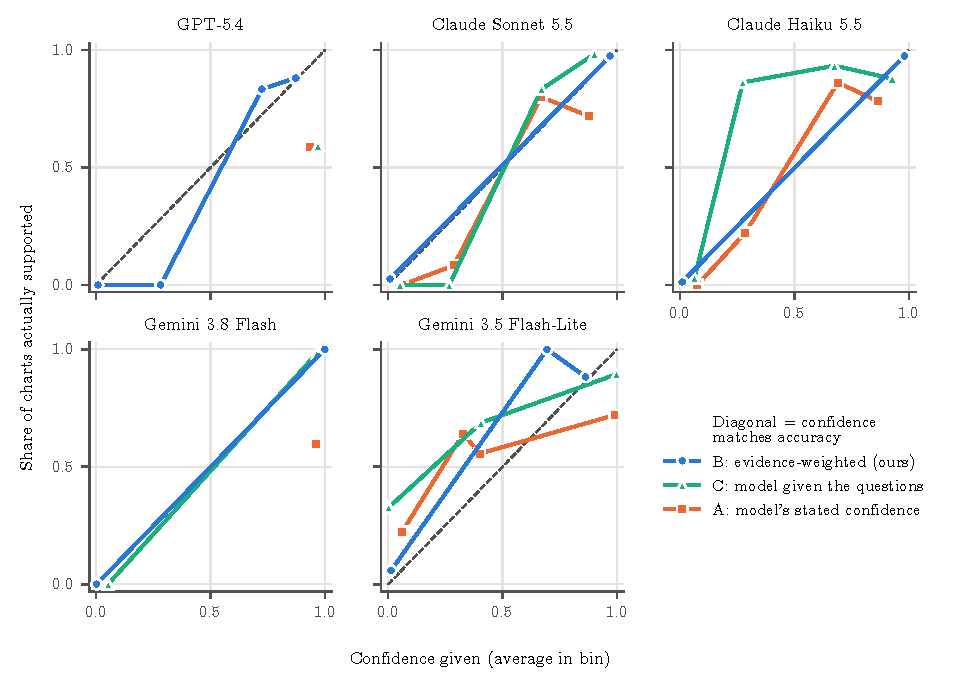
\includegraphics[width=\textwidth]{figures/reliability.pdf}
\caption{Reliability diagrams, study 3 test split. Test charts are grouped into five confidence bins; each point is the average confidence given in a bin (x) against the share of its charts actually supported (y). Bins with fewer than 5 charts are omitted. Points on the dashed diagonal mean the confidence matches the accuracy. GPT-5.4 put almost every chart above 90\% under methods A and C, so each has a single point. On Gemini 3.8 Flash, B and C overlap.}\label{fig:reliability}
\end{figure}

\textbf{When B said 90\% or more, it was right 93--100\% of the time on every model, and its stated confidence matched its accuracy to within one percentage point in each case.} When B gave under 10\%, 0--6\% of the charts were supported. The models' own confidence did not have this property: GPT-5.4 and Gemini 3.8 Flash gave 90\% or more to 149 and 183 of the 200 charts, and only 54\% and 63\% of those were supported. Recalibrating A repairs its average (ECE 0.05--0.11) but cannot repair its ranking, so the recalibrated score crowds into the middle and almost never reaches 90\%: it is honest but not useful for routing.

Giving the model the rubric questions (C) produced honest high confidence on Sonnet and Gemini 3.8 Flash (98--100\% supported above 90\%) but not on the other three models: GPT-5.4 said 97\% and was right 60\% of the time, Flash-Lite said 100\% and was right 89\%, and Haiku put 76 charts in the 10--50\% band of which 70\% were supported. The questions help the model reason; they do not by themselves make its number mean anything. The fitted scoring step does, on every model tested.

Decision metrics tell the same story (Table~\ref{tab:decision}). At a 0.5 cut-off B had the highest $F_{0.5}$ on four models and was within 0.002 of C on Sonnet; at the frozen auto-accept threshold B accepted 59--61\% of all test charts on Sonnet, Haiku and Gemini 3.8 Flash at 96--97\% precision, while recalibrated A accepted at most one chart on any model.

\begin{table}[!htbp]
\centering\small
\caption{Decision quality, study 3 test split (exploratory). Precision, recall and $F_{0.5}$ at a 0.5 cut-off (C's cut-off is the model's own 50\%), and charts auto-accepted at each method's frozen development threshold for 95\% precision (n/a: no development threshold reached 95\%).}\label{tab:decision}
\begin{tabular}{@{}lllll@{}}
\toprule
Model & Method & Precision / recall at 0.5 & $F_{0.5}$ at 0.5 & Auto-accepted (precision) \\
\midrule
\multirow{3}{*}{GPT-5.4} & A recalibrated & 0.613 / 0.650 & 0.620 & n/a \\
 & C & 0.594 / 1.000 & 0.646 & n/a \\
 & B & 0.866 / 0.991 & \textbf{0.888} & 46 (0.935) \\
\midrule
\multirow{3}{*}{Claude Sonnet 5.5} & A recalibrated & 0.738 / 0.889 & 0.764 & n/a \\
 & C & 0.975 / 0.991 & \textbf{0.978} & 124 (0.944) \\
 & B & 0.975 / 0.983 & 0.976 & 119 (0.966) \\
\midrule
\multirow{3}{*}{Claude Haiku 5.5} & A recalibrated & 0.803 / 0.940 & 0.827 & n/a \\
 & C & 0.901 / 0.547 & 0.798 & n/a \\
 & B & 0.975 / 0.991 & \textbf{0.978} & 120 (0.967) \\
\midrule
\multirow{3}{*}{Gemini 3.8 Flash} & A recalibrated & 0.731 / 0.650 & 0.713 & 1 (1.000) \\
 & C & 0.983 / 1.000 & 0.987 & 119 (0.983) \\
 & B & 1.000 / 1.000 & \textbf{1.000} & 122 (0.959) \\
\midrule
\multirow{3}{*}{Gemini 3.5 Flash-Lite} & A recalibrated & 0.720 / 0.658 & 0.706 & n/a \\
 & C & 0.903 / 0.556 & 0.802 & n/a \\
 & B & 0.889 / 0.957 & \textbf{0.902} & n/a \\
\bottomrule
\end{tabular}
\end{table}

\FloatBarrier
\subsection{Tuning the questions, not the model}\label{sec:results-tuning}

Study 2 applied the frozen study-1 pipeline to harder charts. On its first 100 charts B still beat stated confidence by a wide margin (AUROC 0.932 against 0.470 for GPT-5.4; 0.979 against 0.731 for Gemini 3.8 Flash), but it was blind to family F: a visit with a nurse only, an unsigned note, or an e-consult with no patient seen satisfies every question of the six-question rubric. The frozen B gave these 15 charts an average score of 0.94 (GPT-5.4) and 0.99 (Gemini 3.8 Flash) and would have auto-accepted 40\% and 100\% of them. The failure was visible in the evidence trail: every high score came with verified quotes for diabetes, CKD and a plan line, and none for a qualifying encounter or signature, because no question asked for one.

Rubric version 3 added two gates drawn from risk-adjustment rules, R1 (face-to-face visit with an MD, DO, NP or PA) and R2 (signed with a credential), and refined the guidance for borderline wording; weights were refitted on development data. No model was changed. On the study-3 test split, \textbf{B scored every one of the 26 family-F charts as unsupported on all five models} (0 wrong at 0.5). C, which received the same two questions, got 25 of 26 wrong on GPT-5.4 and 4 of 26 on Flash-Lite. Table~\ref{tab:families} gives the errors by family.

\begin{table}[!htbp]
\centering\small
\caption{Charts wrong at a 0.5 cut-off, B / C, by family (study 3 test). Families A--E are easier; F lies outside the pilot rubric; G is borderline ``addressed'' wording; H is the hard cases.}\label{tab:families}
\begin{tabular}{@{}lcccccccc@{}}
\toprule
Model & A (32) & B (27) & C (21) & D (15) & E (15) & F (26) & G (39) & H (25) \\
\midrule
GPT-5.4 & 3 / 14 & 0 / 0 & 0 / 12 & 2 / 9 & 0 / 0 & \textbf{0} / 25 & 9 / 9 & 5 / 11 \\
Claude Sonnet 5.5 & 2 / 0 & 0 / 0 & 0 / 0 & 0 / 0 & 0 / 0 & \textbf{0} / 0 & 1 / 2 & 2 / 2 \\
Claude Haiku 5.5 & 1 / 11 & 1 / 10 & 0 / 4 & 0 / 5 & 0 / 4 & \textbf{0} / 0 & 0 / 19 & 2 / 7 \\
Gemini 3.8 Flash & 0 / 0 & 0 / 0 & 0 / 0 & 0 / 1 & 0 / 0 & \textbf{0} / 0 & 0 / 1 & 0 / 0 \\
Gemini 3.5 Flash-Lite & 1 / 8 & 1 / 12 & 1 / 2 & 0 / 2 & 0 / 5 & \textbf{0} / 4 & 11 / 19 & 5 / 7 \\
\bottomrule
\end{tabular}
\end{table}

The remaining errors sit where the rubric's wording is hardest to apply. Family G (borderline ``addressed'') holds most of B's errors on GPT-5.4 (9) and Flash-Lite (11): the typical errors, seen in development data, were reading ``see nephrology note'' as CKD addressed and missing a medication change made for kidney function, despite explicit guidance on both. Each such error is visible as a specific wrong answer to Q4 with its quote, so the fix is a targeted change to one question's guidance, tested on development data.

\FloatBarrier
\subsection{Inexpensive models}\label{sec:results-cost}

The design pattern moves the judgment from the model to the questions and the fitted weights, so a smaller model only has to read accurately. Table~\ref{tab:cost} compares the two inexpensive models with the frontier models.

\begin{table}[!htbp]
\centering\footnotesize\setlength{\tabcolsep}{4pt}
\caption{Inexpensive and frontier models, study 3 test split. Tokens are for development plus test (1,650 + 2,200 calls); output includes thinking tokens. Costs at list prices where recorded.}\label{tab:cost}
\begin{tabular}{@{}lccccl@{}}
\toprule
Model & B AUROC & B ECE & B 90\%+: said $\rightarrow$ actual & Best A AUROC & Tokens in / out (cost) \\
\midrule
Claude Sonnet 5.5 & 0.987 & 0.021 & 97\% $\rightarrow$ 98\% & 0.715 & 10.4M / 2.3M (\$43.82) \\
Claude Haiku 5.5 & \textbf{0.994} & \textbf{0.014} & 98\% $\rightarrow$ 98\% & 0.772 & 10.1M / 3.6M (\$2.82) \\
\midrule
Gemini 3.8 Flash & 1.000 & 0.002 & 100\% $\rightarrow$ 100\% & 0.647 & 6.7M / 4.1M \\
Gemini 3.5 Flash-Lite & 0.897 & 0.050 & 93\% $\rightarrow$ 93\% & 0.692 & 6.8M / 1.0M \\
\midrule
GPT-5.4 & 0.926 & 0.037 & 93\% $\rightarrow$ 93\% & 0.593 & --- \\
\bottomrule
\end{tabular}
\end{table}

Claude Haiku 5.5 with EWC matched or exceeded Claude Sonnet 5.5 with EWC on every measure, at about one fifteenth of the cost, and passed all four pre-registered checks, the only model to do so. Its extraction was among the most accurate of the five models (macro-$F_1$ at least 0.969 on every question). Gemini 3.5 Flash-Lite, which does not think by default and produced a quarter of Gemini 3.8 Flash's output tokens, reached AUROC 0.897 with EWC, above the stated confidence of every model tested (best 0.772), and its 90\%+ scores were right 93\% of the time. It was not accurate enough to auto-accept at 95\% precision, and its weakest family was the borderline wording of family G (AUROC 0.456). An inexpensive model with the pattern was therefore more trustworthy than any frontier model's own confidence; whether it is good enough to automate depends on the model and is measurable on development data before deployment, as the Flash-Lite threshold showed.

\FloatBarrier
\subsection{Extraction, faithfulness and reproducibility}

Extraction was scored against the intended answers recorded by the generator. Macro-$F_1$ was at least 0.97 on every question for Haiku and Gemini 3.8 Flash. The lowest scores were on Q2 (eGFR below 60 on two results 90 or more days apart; GPT-5.4 0.857, Sonnet 0.847, Flash-Lite 0.743), mostly date arithmetic around the 90-day boundary, and on R2 (signature; GPT-5.4 0.895, Sonnet 0.866, Flash-Lite 0.848), where these models answered ``no'' to R2 for a note signed by a nurse, merging the provider rule into the signature rule. That merge does not change the outcome, because R1 fails on the same chart.

Quote verification failed for 0.0\% (GPT-5.4, Sonnet), 0.1\% (Haiku, Gemini 3.8 Flash) and 0.5\% (Flash-Lite) of yes and no answers, and flagged 0, 0, 0, 1 and 6 test charts for human review. The median standard deviation of B's score across five extraction runs of the same chart was 0.000 on every model, against 0.000--0.034 for stated confidence. Verification therefore remained largely untested in these studies: the models quoted accurately even from notes with format noise.

\FloatBarrier
\subsection{Secondary views and ablations}\label{sec:results-weights}

Table~\ref{tab:ablations} reports views computed from the same calls (exploratory, no pass marks).

\begin{table}[!htbp]
\centering\footnotesize\setlength{\tabcolsep}{4pt}
\caption{Secondary views, study 3 test split: AUROC / ECE. Self-consistency is the share of the five stated-confidence runs that call the chart supported. Expert weights are the illustrative weights of Table~\ref{tab:rubric}, unfitted.}\label{tab:ablations}
\begin{tabular}{@{}lccccc@{}}
\toprule
View & GPT-5.4 & Sonnet 5.5 & Haiku 5.5 & Gemini 3.8 Flash & Flash-Lite \\
\midrule
B, fitted weights & 0.926 / 0.037 & 0.987 / 0.021 & 0.994 / 0.014 & 1.000 / 0.002 & 0.897 / 0.050 \\
Self-consistency & 0.588 / 0.445 & 0.873 / 0.104 & 0.879 / 0.111 & 0.890 / 0.095 & 0.650 / 0.326 \\
B, expert weights & 0.900 / 0.093 & 0.973 / 0.128 & 0.982 / 0.117 & 0.990 / 0.123 & 0.879 / 0.149 \\
B without quote verification & 0.926 / 0.037 & 0.987 / 0.021 & 0.994 / 0.010 & 1.000 / 0.002 & 0.919 / 0.041 \\
B with two-way answers & 0.921 / 0.033 & 0.983 / 0.027 & 0.989 / 0.014 & 0.988 / 0.002 & 0.894 / 0.029 \\
\bottomrule
\end{tabular}
\end{table}

\begin{itemize}
  \item \textbf{Expert weights already rank well; fitting calibrates.} The unfitted illustrative weights reached AUROC 0.879--0.990, close to the fitted weights, but ECE 0.093--0.149. The two-stage use in Section~\ref{sec:bayes} (expert weights on day one, fitted weights once labels exist) is supported.
  \item \textbf{Three-way answers help ranking slightly.} Collapsing \textit{no} and \nd{} lowered AUROC on all five models, by 0.003 to 0.012; calibration was mixed. In study 1, the same ablation cut Gemini 3.8 Flash's auto-accept coverage from 45\% to 0\%.
  \item \textbf{Quote verification changed little.} With so few failed quotes, removing verification left B unchanged on three models; on Flash-Lite it raised AUROC from 0.897 to 0.919, because some answers downgraded by failed quotes had in fact been correct. Verification is a safeguard against invented evidence; these studies did not produce enough invented evidence to measure its value.
  \item \textbf{Letting the LLM compute the score} was tested in study 1 only: given the fitted weights, GPT-5.4's own arithmetic ranked as well as the code (AUROC 0.974 against 0.969) but was far worse calibrated (ECE 0.197 against 0.009); Gemini 3.8 Flash matched the code.
\end{itemize}

\paragraph{Fitted weights are not evidence strengths.} The fitted weights (Table~\ref{tab:weights}) put almost all the signal on Q4 (addressed this visit) and the contradiction answer of Q3 (another cause), which matches how the labels were defined. Q1 (stage documented) received a negative weight on every model. This does not mean a documented stage counts against the code: in these charts a stage appears in many unsupported notes (a staged CKD entry in a problem list that is not addressed), and once Q4 is in the model, ``stage documented'' mostly marks those notes. This is consequence 4 of Section~\ref{sec:bayes} in practice: jointly fitted weights share credit among correlated answers and should be read as a scoring device, while the audit trail is the answers and quotes. The selected regularization strength was large for the strongest extractors ($C=31.6$ for Sonnet and Haiku, 316 for Gemini 3.8 Flash), a sign that the answers nearly separate the classes on these data.

\begin{table}[!htbp]
\centering\small
\caption{Weights fitted on study 3 development data (log-odds; \nd{} is the zero point; Q1 and Q4 have no ``no'' answer).}\label{tab:weights}
\begin{tabular}{@{}lrrrrrrrr@{}}
\toprule
Model & $w_0$ & Q1 yes & Q2 yes & Q2 no & Q3 yes & Q3 no & Q4 yes & $C$ \\
\midrule
GPT-5.4 & $-0.15$ & $-1.29$ & 0.56 & $-1.11$ & 0.90 & $-2.19$ & 2.44 & 3.2 \\
Claude Sonnet 5.5 & $-0.61$ & $-4.88$ & 2.29 & 1.42 & 0.11 & $-6.73$ & 7.79 & 31.6 \\
Claude Haiku 5.5 & $-0.04$ & $-5.33$ & 1.84 & $-0.35$ & 1.74 & $-6.50$ & 7.83 & 31.6 \\
Gemini 3.8 Flash & $-3.08$ & $-2.84$ & $-0.14$ & $-1.47$ & 0.80 & $-10.43$ & 12.54 & 316 \\
Gemini 3.5 Flash-Lite & $-2.15$ & $-0.08$ & 0.10 & $-0.66$ & 0.99 & $-1.58$ & 3.72 & 3.2 \\
\bottomrule
\end{tabular}
\end{table}

\FloatBarrier
\subsection{Earlier studies}

\paragraph{Study 1 (pilot).} 200 charts in 13 scenarios (140 development, 60 test), the six-question rubric, GPT-5.4 and Gemini 3.8 Flash. One rubric revision on development data (version 2) told the models when to answer \nd{} rather than \textit{no}, which raised GPT-5.4's Q4 macro-$F_1$ from 0.574 to 1.000. On test, B reached AUROC 0.969 and ECE 0.009 (GPT-5.4) and 0.979 and 0.016 (Gemini 3.8 Flash), against recalibrated stated confidence at 0.571 and 0.107, and 0.669 and 0.120. GPT-5.4's raw stated confidence had ECE 0.514. The only wrongly accepted chart for both models was a copied-forward note whose label was itself flagged as debatable. All pilot charts turned out to be close to separable by the rubric, which motivated the harder charts of study 2.

\paragraph{Study 2 (transfer test).} The frozen pilot pipeline on 300 harder charts, without refitting. Stage 1 (100 charts) showed B still far ahead of stated confidence and of criteria-guided confidence for GPT-5.4 (AUROC 0.932 against 0.470 and 0.441), and ahead of stated confidence for Gemini 3.8 Flash (0.979 against 0.731; C 0.961), but blind to family F, as described in Section~\ref{sec:results-tuning}. The study was stopped there, as its pre-registration allowed, and its 200 unseen charts became most of study 3's test split.

\FloatBarrier
\subsection{Deviations from the plan}

Self-consistency used the five stated-confidence runs instead of separate calls, to save cost. A tolerant JSON parse was declared before the first call for Claude Haiku 5.5 and Gemini 3.5 Flash-Lite, after one test call returned a raw control character inside a string. For Claude Sonnet 5.5, the development evaluation, the addendum freeze and the test collection were started together by mistake; the fitting is deterministic and all nine frozen files matched the development fit, so the test used the intended weights. Study 2's stage 2 was not run. The confidence-versus-accuracy table, the decision metrics at 0.5 and the reliability figure were computed after the test and are exploratory.

% ---------------------------------------------------------------------------
\section{Generalizing across use cases}\label{sec:general}

The rubric changes with every use case; the pipeline, the scoring theory and the protocol do not (Table~\ref{tab:usecases}).

\begin{table}[!htbp]
\centering\small
\caption{The same structure applied to other decisions.}\label{tab:usecases}
\begin{tabularx}{\textwidth}{@{}p{2.4cm}p{2.6cm}LL@{}}
\toprule
Use case & Output being scored & Example gate & Example weighted question \\
\midrule
Diagnosis coding & An ICD-10-CM code & Condition documented in a face-to-face encounter & Condition treated or monitored this visit \\
Prior authorization & An approve recommendation & Diagnosis on the policy's covered list & Six weeks of failed conservative therapy documented \\
Post-pay overpayment & An overpayment finding & Claim falls under the cited policy & Billed units exceed the documented service \\
Clinical-trial matching & A patient-trial match & Age within the inclusion range & Lab values within the inclusion window \\
\bottomrule
\end{tabularx}
\end{table}

Prior authorization is the closest analogue. Teams already turn policy lines into questions and have an LLM answer them with citations. Prior authorization combines the answers with AND/OR logic into approve, deny or pend. This method keeps that logic for gates and adds weighted questions for graded confidence, so an existing policy-to-question engine can be reused with only the combination layer changed. The same criterion-level structure supports monitoring such a system in production~\cite{zeinoun}.

\paragraph{Scaling the rubrics.} Writing a separate rubric for each of roughly 70,000 ICD-10-CM codes is not feasible. Rubrics are layered instead:
\begin{enumerate}
  \item \textbf{Generic layer:} questions that apply to every output of the use case (for coding, the MEAT criteria and encounter-type rules, such as R1 and R2 in the experiments).
  \item \textbf{Family layer:} shared logic for a category (for diabetes with complications: condition, complication, link).
  \item \textbf{Code layer:} overrides for high-value or high-error codes only.
\end{enumerate}
The layering is also a statistical device. A rare code with 15 labeled examples cannot support its own weights, but it can borrow its family's weights and adjust slightly: partial pooling, as in hierarchical regression. Effort goes first to the small set of codes that drive most financial value and audit risk. Candidate questions can be drafted by an LLM from official coding guidelines and then reviewed by certified coders, with every rubric versioned.

% ---------------------------------------------------------------------------
\section{Extensions for improving accuracy}

The method is a way to measure confidence; the extensions below aim to make what it measures more accurate or cheaper to obtain. None was used in the experiments. They apply to any use case, not only medical coding.
\begin{itemize}
  \item \textbf{Semantic verification of evidence.} Exact-quote matching shows that the evidence exists, not that it supports the answer. A second model, ideally from a different model family, could judge whether each quote, shown with its surrounding text and section, supports, fails to support or contradicts the answer. This is the attribution-checking problem studied for LLM-generated text~\cite{rashkin,gao,yue}, and it corresponds to the conservative AI critic proposed for prior-authorization monitoring in~\cite{zeinoun}. The errors that remained in the experiments were of this kind: real quotes, such as ``see nephrology note'', read as supporting an answer they do not support.
  \item \textbf{Decision-relevant verification.} Because scoring is deterministic and nearly free, costly checks can be limited to answers whose removal would move an output across a routing threshold. A random sample of skipped checks would still be run, to measure how often skipping is wrong.
  \item \textbf{Cost controls.} Asking all questions in one call per document, caching the fixed instructions and rubric, requiring compact structured output, and batch processing all reduce cost without changing the scoring. The experiments suggest a larger lever: a smaller model inside the pattern (Section~\ref{sec:results-cost}).
  \item \textbf{Evidence retrieval across documents.} Many reviews span several documents, such as earlier visits or separate lab reports. An orchestrating agent could fetch additional records when evidence is missing, with every action logged. The scoring and routing would stay fixed, so the score remains reproducible from the logged evidence.
  \item \textbf{Production monitoring.} Once deployed, labels are scarce. The method's intermediate outputs give label-free signals in the sense of~\cite{zeinoun}: the rate of each answer per question, the quote-failure rate, the gate-failure rate and the share of charts flagged for review. A shift in these signals shows where the system changed, though not whether it is wrong. Periodic human review of a targeted sample then gives labels to recheck calibration and criterion-level extraction quality.
\end{itemize}

% ---------------------------------------------------------------------------
\section{Limitations}

\paragraph{Limitations of the experiments.}
\begin{itemize}
  \item \textbf{Synthetic charts.} All notes were generated from phrase banks and edited templates. Real notes are longer, messier and more varied, and real documentation errors are not drawn from a fixed list of scenarios.
  \item \textbf{Labels favor the method by construction.} The labels follow mostly from facts the rubric asks about, so a model that answers the questions correctly will score well. Method C received the same questions to keep the comparison fair, and the method's value on real charts depends on how well a rubric captures the real labeling rules.
  \item \textbf{No certified coder.} The label rules were set by the study lead with AI assistance, and one reviewer checked 74 charts with an AI reading aid. A Gemini model (3.1 Pro) assisted the review and Gemini models were tested.
  \item \textbf{Same-family generation.} The charts were generated with Claude, and two Claude models were tested; their results may be favored.
  \item \textbf{Prevalence.} About 58\% of test charts are supported, far above a real population. The intercept can be shifted for deployment (Appendix~\ref{app:algo}), but calibration must be rechecked on real data.
  \item \textbf{Small, easy-to-separate data.} About 100 gate-passing development charts per model fitted the weights, and the strongest extractors nearly separated the classes. Bootstrap intervals are reported, but 200 test charts cannot resolve small differences, and one candidate code was tested.
  \item \textbf{Verification barely exercised.} Models almost never quoted text that was not in the note, so the quote check's value against invented evidence is not measured here.
  \item \textbf{Added models.} Three of the five models were added after the pre-registration, each under its own addendum filed before its first call; their results are confirmatory only in that narrower sense.
\end{itemize}

\paragraph{Limitations of the method.}
\begin{itemize}
  \item \textbf{Documented is not the same as true.} The score measures how well the source supports an output. Cloned or copied-forward notes can satisfy every question.
  \item \textbf{Extraction errors remain.} Verification catches invented quotes, not real quotes misread. A quote can exist and still not support the answer; this is where the remaining errors in the experiments came from.
  \item \textbf{Rubric bias.} Questions and expert weights encode their authors' views. Fitting corrects the weights, not missing questions, as family F showed before R1 and R2 were added.
  \item \textbf{Guideline interpretation.} The rubric encodes one reading of the coding guidelines. Coders, payers and auditors can read edge cases differently, such as a missing CKD stage or a copied-forward note, and the mapping needs review by certified coders.
  \item \textbf{Label cost.} Calibration needs coder-labeled data per code family, and labels themselves carry disagreement.
  \item \textbf{Drift.} Documentation habits, coding guidelines and risk-adjustment models change, so weights must be refitted and rubrics re-versioned.
  \item \textbf{Gaming.} If providers learn the rubric, documentation may be written to satisfy it rather than to describe care.
\end{itemize}

% ---------------------------------------------------------------------------
\section{Conclusion}

A confidence number has meaning only when it is computed from checked evidence and tested against outcomes. Evidence-weighted confidence does both: the LLM supplies cited answers to rule-derived questions, code verifies and scores them, and logistic regression turns the score into a calibrated probability. The additive scoring is exact Bayesian updating in log-odds form.

On synthetic E11.22 charts and five models, the pattern did what it was designed to do. Its confidence meant what it said: charts it scored 90\% or more were supported 93--100\% of the time on every model, while the models' own 93--99\% was right 54--72\% of the time. It ranked charts far better than the models' own confidence on every model, and it was the best-calibrated method on every model. A failure found on new charts was fixed by adding two questions, without touching the models. And an inexpensive model inside the pattern matched the best frontier model at a fraction of the cost. Giving the model the questions without the scoring step was enough for the strongest models to rank well, but not to make their confidence trustworthy across models.

The next step is real charts labeled by certified coders, more codes, and a semantic check of the quotes, which is where the remaining errors lie.

% ---------------------------------------------------------------------------
\begin{thebibliography}{99}\small
\bibitem{xiong} Miao Xiong, Zhiyuan Hu, Xinyang Lu, Yifei Li, Jie Fu, Junxian He, and Bryan Hooi. Can LLMs express their uncertainty? An empirical evaluation of confidence elicitation in LLMs. In \emph{International Conference on Learning Representations (ICLR)}, 2024. \url{https://arxiv.org/abs/2306.13063}.
\bibitem{leng} Jixuan Leng, Chengsong Huang, Banghua Zhu, and Jiaxin Huang. Taming overconfidence in LLMs: Reward calibration in RLHF. In \emph{International Conference on Learning Representations (ICLR)}, 2025. \url{https://arxiv.org/abs/2410.09724}.
\bibitem{soroush} Ali Soroush et al. Large language models are poor medical coders: Benchmarking of medical code querying. \emph{NEJM AI}, 1(5), 2024. doi: 10.1056/AIdbp2300040.
\bibitem{platt} John C. Platt. Probabilistic outputs for support vector machines and comparisons to regularized likelihood methods. In A.~Smola, P.~Bartlett, B.~Sch\"olkopf, and D.~Schuurmans, editors, \emph{Advances in Large Margin Classifiers}. MIT Press, Cambridge, MA, 2000.
\bibitem{checkeval} Yukyung Lee, Joonghoon Kim, Jaehee Kim, Hyowon Cho, Jaewook Kang, Pilsung Kang, and Najoung Kim. CheckEval: A reliable LLM-as-a-judge framework for evaluating text generation using checklists. In \emph{Proceedings of the 2025 Conference on Empirical Methods in Natural Language Processing (EMNLP)}, 2025. \url{https://arxiv.org/abs/2403.18771}.
\bibitem{cbm} Pang Wei Koh, Thao Nguyen, Yew Siang Tang, Stephen Mussmann, Emma Pierson, Been Kim, and Percy Liang. Concept bottleneck models. In \emph{Proceedings of the 37th International Conference on Machine Learning (ICML)}, volume 119 of PMLR, pages 5338--5348, 2020. \url{https://proceedings.mlr.press/v119/koh20a.html}.
\bibitem{good} I.~J. Good. \emph{Probability and the Weighing of Evidence}. Griffin, London, 1950.
\bibitem{zeinoun} Issam Zeinoun. Beyond accuracy: A risk-driven architecture for monitoring AI in prior authorization. Zenodo, 2026. \url{https://doi.org/10.5281/zenodo.23628695}. Also posted on LinkedIn, September 2026.
\bibitem{guidelines} Centers for Medicare \& Medicaid Services and National Center for Health Statistics. ICD-10-CM official guidelines for coding and reporting, FY 2027, 2026. \url{https://ftp.cdc.gov/pub/Health_Statistics/NCHS/Publications/ICD10CM/2027/ICD-10-CM-October-1-2026-FY27-Guidelines.pdf}. Effective October 1, 2026.
\bibitem{tabular} Centers for Medicare \& Medicaid Services. 2027 ICD-10-CM code tables, tabular and index, 2026. \url{https://www.cms.gov/files/zip/2027-code-tables-tabular-index.zip}. Tabular List entry for E11.22, Type 2 diabetes mellitus with diabetic chronic kidney disease, and its instructional notes.
\bibitem{rashkin} Hannah Rashkin, Vitaly Nikolaev, et al. Measuring attribution in natural language generation models. \emph{Computational Linguistics}, 49(4), 2023. \url{https://aclanthology.org/2023.cl-4.2}.
\bibitem{gao} Tianyu Gao, Howard Yen, Jiatong Yu, and Danqi Chen. Enabling large language models to generate text with citations. In \emph{Proceedings of the 2023 Conference on Empirical Methods in Natural Language Processing (EMNLP)}, pages 6465--6488, 2023. \url{https://aclanthology.org/2023.emnlp-main.398}.
\bibitem{yue} Xiang Yue, Boshi Wang, Ziru Chen, Kai Zhang, Yu Su, and Huan Sun. Automatic evaluation of attribution by large language models. In \emph{Findings of the Association for Computational Linguistics: EMNLP 2023}, 2023. \url{https://arxiv.org/abs/2305.06311}.
\end{thebibliography}

% ---------------------------------------------------------------------------
\appendix
\section{Algorithm specification}\label{app:algo}

The pipeline has two paths. Inference scores one chart with a frozen weight table; training fits that table from labeled charts. Extraction is the only step that uses an LLM; everything after it is deterministic code.

\FloatBarrier
\subsection{Notation}
\begin{itemize}
  \item $T$: the source document (chart text).
  \item Gate questions $g_1,\dots,g_k$ and weighted questions $q_1,\dots,q_m$, each answered from the set \{yes, no, \nd\}.
  \item Labeled data $D=\{(T_i,y_i)\}_{i=1}^{N}$, with $y_i=1$ if the candidate code is supported and 0 otherwise.
\end{itemize}

\FloatBarrier
\subsection{Inference}

\begin{algorithm}[h]
\caption{Scoring one document with a frozen weight table}
\begin{algorithmic}[1]
\Require document $T$; gates $G$; weighted questions $Q$; weights $(w_0,\mathbf{w})$
\State $\{(a_j,s_j)\}\gets$ \Call{LLM-Extract}{$T,G\cup Q$} \Comment{answers and verbatim quotes; weights never shown}
\State $\mathit{review}\gets$ false
\For{all questions $j$ with $a_j\in\{\text{yes},\text{no}\}$}
  \If{\Call{Normalize}{$s_j$} is not a substring of \Call{Normalize}{$T$}}
    \If{$j\in G$ or $a_j=\text{no}$} \State $\mathit{review}\gets$ true \EndIf
    \State $a_j\gets$ \nd \Comment{downgrade and log}
  \EndIf
\EndFor
\If{$\exists g\in G: a_g\neq\text{yes}$} \State \Return $p=0$, $\mathit{review}$ \EndIf
\State $\mathbf{x}\gets$ indicators $(\ind[a_q=\text{yes}],\ind[a_q=\text{no}])_{q\in Q}$ \Comment{\nd{} is the reference}
\State $z\gets w_0+\mathbf{w}^\top\mathbf{x}$;\quad $p\gets 1/(1+e^{-z})$
\State log answers, quotes, verification results, rubric and weight versions, $z$, $p$
\State \Return $p$, $\mathit{review}$ \Comment{flagged charts are never auto-accepted}
\end{algorithmic}
\end{algorithm}

Verification is a plain substring test after normalization (case folding, unified quote and dash characters, and collapsed whitespace); no regular expressions or fuzzy matching are used. Reference coding matters for interpretation. With one indicator per answer plus an intercept, a question's three indicators always sum to 1, so the weights are not uniquely determined: a constant can move between them and the intercept without changing any prediction. With \nd{} as the baseline, each weight is the change in log-odds relative to the source being silent. The illustrative weights in Section~\ref{sec:example} use the same convention. The probability is
\begin{equation}
z=w_0+\sum_{j=1}^{d}w_jx_j,\qquad P(Y=1\mid\mathbf{x})=\sigma(z)=\frac{1}{1+e^{-z}},\qquad d\le 2m.
\end{equation}

\FloatBarrier
\subsection{Training}

Only charts that pass every gate enter training, because gate failures are scored 0 by rule and carry no information about the weights. The weights minimize L2-regularized log-loss, with the intercept $w_0$ unpenalized:
\begin{equation}\label{eq:obj}
\min_{w_0,\mathbf{w}}\ \frac12\|\mathbf{w}\|_2^2 + C\sum_{i=1}^{N}\Big[-y_i\log\sigma(z_i)-(1-y_i)\log\big(1-\sigma(z_i)\big)\Big],\qquad z_i=w_0+\mathbf{w}^\top\mathbf{x}_i.
\end{equation}
\begin{itemize}
  \item Log-loss is a proper scoring rule: its expected value is lowest only when the predicted probabilities are the true ones. That is why it serves as both the training objective and the model-selection criterion.
  \item The L2 penalty keeps weights finite when an indicator perfectly separates the classes, which is likely in small or synthetic datasets. Without it, the fitted weights would grow without bound.
  \item $C$ is the inverse penalty strength. Smaller $C$ gives smaller, more conservative weights; larger $C$ fits the training data more closely.
  \item The intercept is not penalized, so the prior is not pulled toward 50\%. The objective is convex, so any standard solver (for example L-BFGS) reaches the same unique solution.
\end{itemize}

\paragraph{Gradient.} Write $L(w_0,\mathbf{w})$ for the objective in Equation~\eqref{eq:obj}. Because the derivative of the sigmoid cancels against the log-loss, the gradient is short:
\begin{equation}
\frac{\partial L}{\partial w_j}=w_j+C\sum_{i=1}^{N}\big(\sigma(z_i)-y_i\big)x_{ij},\qquad
\frac{\partial L}{\partial w_0}=C\sum_{i=1}^{N}\big(\sigma(z_i)-y_i\big).
\end{equation}
A plain gradient-descent iteration moves every weight a small step $\eta$ against its gradient:
\begin{equation}
\mathbf{w}\gets\mathbf{w}-\eta\nabla_{\mathbf{w}}L,\qquad w_0\gets w_0-\eta\frac{\partial L}{\partial w_0}.
\end{equation}
Each weight therefore moves in proportion to the prediction error $\sigma(z_i)-y_i$, summed over the charts where its answer appeared. If charts with Q3 = yes keep scoring lower than their labels, the Q3-yes weight rises. The penalty term $w_j$ pulls every weight back toward 0; the intercept has no such term, so the prior is not shrunk. The reference implementation uses L-BFGS, a faster method driven by the same gradient. Because the objective is convex, it has a single minimum, so gradient descent, L-BFGS and any other standard solver reach the same weight table from any starting point.

The selection of $C$ in Algorithm~\ref{alg:fit} is $k$-fold cross-validated grid search, not nested cross-validation. Nested cross-validation adds an outer loop that estimates how well the whole selection procedure generalizes; here the untouched test split plays that role. When the loss keeps improving as $C$ grows, the weights reflect the penalty rather than measured evidence strength.

\FloatBarrier
\subsection{Adjusting the prior for deployment}

The fitted intercept reflects the share of positive charts in the training data. When the deployment population has a different share, shift the intercept:
\begin{equation}
w_0'=w_0+\operatorname{logit}(\pi_{\text{deploy}})-\operatorname{logit}(\pi_{\text{train}}),\qquad \operatorname{logit}(p)=\log\frac{p}{1-p}.
\end{equation}
Here $\pi$ is the share of positive charts among those that pass the gates. The correction assumes the evidence looks the same within each class in both settings (label shift only), so calibration must still be checked on a deployment sample. This matters for the experiments: their synthetic charts are 44--58\% positive, far above a real diabetic population.

\begin{algorithm}[h]
\caption{Fitting the weight table on the development split}\label{alg:fit}
\begin{algorithmic}[1]
\Require development charts with verified answers and labels; target grid $\mathcal{C}=\{10^{-3},10^{-2.5},\dots,10^{3}\}$ (13 values)
\State keep only charts whose gate answers are all yes; encode $\mathbf{x}_i$ as in Algorithm 1
\For{all $C\in\mathcal{C}$}
  \For{$r=1,\dots,10$} \Comment{repeated, stratified 5-fold CV; a patient's charts stay in one fold}
    \For{each fold $f=1,\dots,5$}
      \State fit Equation~\eqref{eq:obj} on the other four folds; record log-loss on fold $f$
    \EndFor
  \EndFor
  \State $\bar L(C)\gets$ mean log-loss over the 50 fits
\EndFor
\State $C^\star\gets\arg\min_C \bar L(C)$ \Comment{or the one-standard-error rule, fixed in advance}
\If{$C^\star$ lies at the edge of $\mathcal{C}$}
  \State extend the grid; if the loss keeps improving, report that the indicators separate the classes
\EndIf
\State refit on all development charts with $C^\star$; freeze and version the weight table
\State score the held-out test split once (Section~\ref{sec:protocol})
\end{algorithmic}
\end{algorithm}

\FloatBarrier
\subsection{Reference implementation}

A minimal Python version of the encoding and of Algorithm~\ref{alg:fit}, using scikit-learn (tested with version 1.9.1, whose L-BFGS solver leaves the intercept unpenalized). The experiments use the same procedure with the gates of rubric version 3 (G1, G2, R1, R2):
\begin{lstlisting}[language=Python]
import numpy as np
from sklearn.linear_model import LogisticRegression
from sklearn.model_selection import GridSearchCV, RepeatedStratifiedKFold

WEIGHTED_QS = ["Q1", "Q2", "Q3", "Q4"]
GATES = ["G1", "G2"]

def encode(answers):
    """Verified answers -> indicators; not_documented is the reference category."""
    return [int(answers[q] == v) for q in WEIGHTED_QS for v in ("yes", "no")]

def fit_weights(dev_answers, dev_labels):
    keep = [i for i, a in enumerate(dev_answers) if all(a[g] == "yes" for g in GATES)]
    X = np.array([encode(dev_answers[i]) for i in keep])
    y = np.array([dev_labels[i] for i in keep])
    search = GridSearchCV(
        LogisticRegression(solver="lbfgs", max_iter=10_000),  # L2 by default
        param_grid={"C": np.logspace(-3, 3, 13)},
        scoring="neg_log_loss",
        cv=RepeatedStratifiedKFold(n_splits=5, n_repeats=10, random_state=0),
        refit=True,
    )
    search.fit(X, y)
    model = search.best_estimator_
    names = [f"{q}_{v}" for q in WEIGHTED_QS for v in ("yes", "no")]
    table = {"intercept": float(model.intercept_[0]),
             **dict(zip(names, map(float, model.coef_[0])))}
    return table, search.best_params_["C"]
\end{lstlisting}

% ---------------------------------------------------------------------------
\section{Rubric version 3}\label{app:rubric}

The rubric used in study 3. Each question is answered yes, no or \nd{} with an exact quote; the guidance is given to the model with the question (abridged here). Method C received the same questions and guidance.

\begin{small}
\noindent\begin{tabularx}{\textwidth}{@{}p{0.6cm}p{1.4cm}L@{}}
\toprule
ID & Role & Question and guidance \\
\midrule
G1 & Gate & \textit{Is type 2 diabetes mellitus documented as a current diagnosis?} Yes for type 2, or diabetes without a type (ICD-10-CM defaults to type 2); insulin use does not change the type. No for type 1, secondary diabetes (drug, chemical, another condition, a procedure such as pancreatectomy), or both type 1 and type 2 without saying which is correct. \\
G2 & Gate & \textit{Is chronic kidney disease documented by the provider as an established diagnosis?} Yes if CKD is diagnosed anywhere, including ESRD or stage 5, or a history of CKD managed at this visit. No if possible, suspected, rule out, ``CKD?'', deferred; if the current assessment questions or defers CKD although the problem list includes it; or if the note elsewhere says there is no kidney disease and does not resolve the contradiction. Not documented for abnormal labs only, ``kidneys OK'', or ``renal involvement'' without the words CKD or chronic kidney disease. \\
R1 & Gate & \textit{Was the patient seen face-to-face, in person, by a physician (MD or DO), nurse practitioner or physician assistant?} No if the visit was with a nurse, dietitian or other staff only, or the patient was not seen (chart review, e-consult). \\
R2 & Gate & \textit{Is the note signed by the clinician with a professional credential?} Yes only if a signature line names the clinician with a credential such as MD, DO, NP, FNP-C or PA-C. No if unsigned, pending signature, or without a credential. \\
Q1 & Weighted & \textit{Is the CKD stage documented?} Yes if a stage (3a, 3b, 4, 5 or ESRD) is stated anywhere, even if sections or labs disagree; otherwise not documented, not no. \\
Q2 & Weighted & \textit{Do the labs show eGFR below 60 on two results at least 90 days apart?} Yes if two results below 60 are dated at least 90 days apart; no only if the most recent eGFR is 60 or above; otherwise not documented. \\
Q3 & Weighted & \textit{Does the provider attribute the CKD to diabetes?} Yes if due to, secondary to or caused by diabetes, or diabetic kidney disease, including diabetes named with another cause or as the likely cause. No if attributed to a different cause instead of diabetes. Not documented if no cause is stated. \\
Q4 & Weighted & \textit{Was the CKD addressed at this encounter (monitored, evaluated, assessed or treated)?} Yes if CKD appears in the assessment and plan with any status, evaluation, plan or treatment, including a copied-forward line (``stable'', ``continue regimen'') or CKD in a list of chronic conditions reviewed in the plan; a medication change because of kidney function counts. Not documented if CKD appears only in the problem list or history, or the plan only refers to another clinician's note (``see nephrology note''). \\
\bottomrule
\end{tabularx}
\end{small}

\paragraph{Materials.} The chart generator, data, rubric, prompts, pre-registrations, freeze records, analysis code and a change log of every decision are in the study repository.

\end{document}
